\documentclass[conference]{IEEEtran}
\ifCLASSINFOpdf
   \usepackage[pdftex]{graphicx}
\else
\fi
\usepackage{amsmath}
\usepackage{stfloats}
\usepackage{verbatim}
\usepackage{multicol}
\hyphenation{op-tical net-works semi-conduc-tor}


\begin{document}
\title{Design of Oversampled ADC Integrators \\ \Large EE240B Project Report}
\author{\IEEEauthorblockN{Emily Naviasky}
\IEEEauthorblockA{Department of EECS, UC Berkeley \\enaviasky@berkeley.edu}
\and
\IEEEauthorblockN{Nathaniel Mailoa}
\IEEEauthorblockA{Department of EECS, UC Berkeley \\nmailoa@eecs.berkeley.edu}
}
\maketitle

\section{Introduction}

We will propose a design for the integrator stages of an oversampled ADC. The design is driven by specifications that include input-referred electronic noise, settling time as well as settling accuracy. We have chosen to use the same integrator architecture for both stages but tune the component values for each stage.\\

\section{System-level Considerations}

We started the design by modeling the ADC as transfer functions. We noticed that since the circuit implements an integration, the first stage should be a lot more carefully designed than the second stage. The input-referred noise transfer function from the output of the first stage is $N_1 = 2(z-1)$ while the second stage has a contribution that is affected by $N_2 = 0.25(z-1)^2$, assuming a second stage gain of 0.5. These transfer functions are also used later to verify the input-referred electronic noise of the circuit.

We estimated that the noise power contribution of the second stage is approximately 1000 times smaller than the first stage. We also noted that if we split the noise of a stage to each phases' noises ($\Phi_1$ and $\Phi_2$), the noise from $\Phi_1$ is integrated along with the signal and is more important than the $\Phi_2$ noise. We use this analysis to size the sampling and feedback capacitors of both integrator stages separately.\\

\section{Integrator Implementation}

Each integrator stage of the oversampled ADC has a gain of 0.5 and has to settle within 0.1\% in 1.8ns wih a +/- 1V differential input. Fig. \ref{fig:int} shows the implementation of the integrator stages.

\begin{figure}[h]
\centering
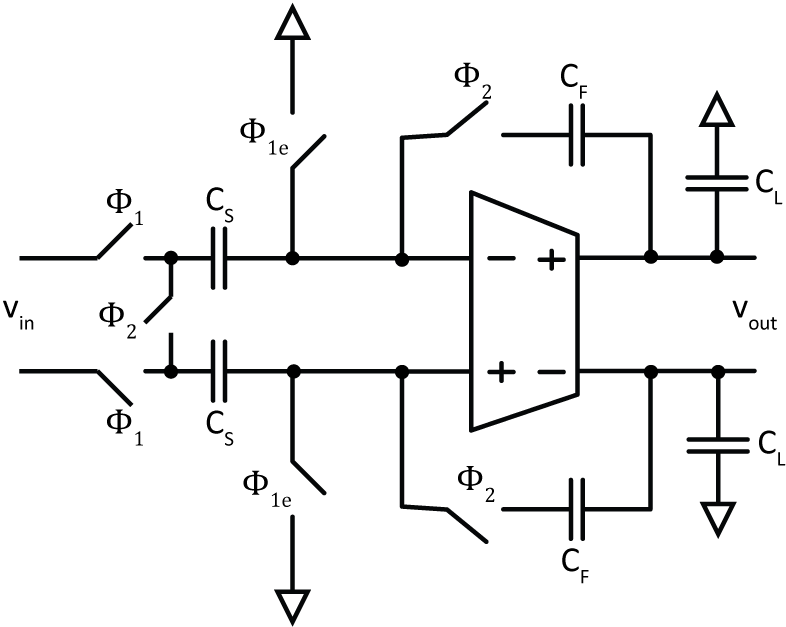
\includegraphics[width=0.75\linewidth]{illus/integrator}
\caption{Switched capacitor integrator}
\label{fig:int}
\end{figure}

During $\Phi_1$, $C_S$ samples the input and during $\Phi_2$ the input is amplified through charge transfer between $C_S$ and $C_F$. The $\Phi_2$ switch connecting the two sampling capacitors is a common mode rejection mechanism, transferring only the differential charge to $C_F$. $C_F$ is connected in the feedback only during the amplification phase $\Phi_2$ and is never reset, thus it integrates the input over time. $C_L$ is the load capacitance; for the first stage this is the the sampling capacitor of the second stage, and for the second stage this is the input capacitance of the comparator.

Since the amplifiers form a second-order integrator, the first amplifier noise dominates the total noise. We begin by choosing $C_S$ from the noise specification and the equation for noise at $\Phi_1$. 

$$N_{\Phi 1} = \frac{kT}{C_S + C_L}$$
$$N_{\Phi 2} = \frac{\alpha}{\beta}\frac{kT}{C_{L,tot}}$$

The value of $C_F$ is easily obtained from the required gain since the gain of the integrator is $C_F/C_S$. We want to budget $3.5 \mu$ $V_{RMS}$ to the noise at $\Phi_1$ per differential input, but the signal bandwidth that we care about is only 100-500kHz and our equation for $N_{\phi 1}$ is over the entire spectrum. Therefore, we need to multiply the noise specification by the Oversampling Ratio, which is $\frac{f_S}{2BW}$. The input referred noise that we want therefore is $N_{\Phi 1}=250 \cdot (3.5)^2 \cdot 10^{-12} V/\sqrt{Hz}$. We rounded the capacitor values up to get some headroom for error.

%IMPT VALS
$$C_S = 1.5pF$$ 
$$C_F = 3pF$$

Our load capacitor is the sampling capacitor of stage 2. We first started at 100fF and iteratively lumped in parasitic capacitances from the OTA with the load capacitor.

We next calculate the $G_m$ of the OTA which is dictated by the unity gain bandwidth necessary to meet the settling time with those capacitors from the settling time requirement since $\omega_u = \frac{G_m}{C_{L,tot}} $. The equation below expresses the dynamic settling error specification assuming a zero, where $\tau$ is the unity gain bandwidth and $\beta=.67$.  

$$t_s = -\tau ln \left(\epsilon_d \left(1-\beta \frac{C_F}{C_F-C_L}\right)\right)$$

We budget half of the error to static error and half to dynamic, so $\epsilon_d = 0.0005$. In addition, we budgeted .8ns of the settling time to slewing and devices in the second branch being pushed out of saturation so the $t_s = 1ns$. This results in a unity gain bandwidth of 1.4G and a required transconductance of $G_m = 10mS$.

Next we calculated the required open loop gain of the amplifier. Since we are budgeting half of the settling error to static error, we require that
$$\frac{1}{T} = \frac{1}{\beta A} = \epsilon_s = 0.0005$$

With a $\beta$ of 0.67, the required open loop gain is 3000, or 70 dB. As a quick check, this results in a required output resistance of $300k\Omega$. Which is a bit high and requires at least cascoding.

With the design parameters, we started by building an ideal OTA using a VCCS. We created a testbench for AC, noise, and transient analysis and ran simulations to make sure the settling time, and noise requirements are met. The noise simulation was a performed with a noise current source from a resistor of value $\frac{\alpha}{G_m}$ inside of the OTA and $10\Omega$ ON resistances in series with all of the switches. However, PSS and PNOISE are not really meant for integrators so we exported the noise density at the output of the integrator to Matlab, then multiplied by the input-refered transfer function from the noise source and then integrated over the signal bandwidth.

With a one stage OTA, the transconductance is limited by the $g_m$ of the input device and we already determined that we need $g_m = 10mS$. Assuming a $V* = .2$, the current required is 1mA. We check that the current is close to that required for the slewing. To avoid slewing for extended periods of time, the current in the input device has to be large enough to charge the load capacitance. Since when the closed loop amplifier is subjected to a step input there is a capacitive divider effect from the input to the output node, the output has to slew more than the maximum single-ended output swing of $0.25V$. Designing for a $1V$ slew in $0.8ns$, with a total load capacitance of $C_{Ltot} = C_L + (1-\beta)C_F = 1.1pF$, the current needed in the input devices is $1.3mA$. Since the required $g_m$ is lower than that, we err on the side of more and use  $1.3mA$. Once it was implemented, we found that the slewing was not as bad as we had feared, and we backed off the current to $1.2mA$. This still gives us a higher unity gain BW than required, which means that we need to be sensitive of our phase margin, but the overestimation is not terrible since the unity gain BW is underestimated by assuming only a single pole system. Finally, in order to settle to $.1\%$ we needed a phase margin of at least 70 degrees. With these design specifications in mind, we began designing our circuit.\\

\section{Design Alternatives}

We started with a telescopic OTA with an NMOS input but quickly realized that there was not enough head room to maintain a common mode output voltage at 0.6V. We moved on to a folded cascode OTA architecture to obtain the necessary headroom. 

The current of the cascode branch is typically about 1.5 time greater than the current flowing through the input devices so the cascode devices stay biased properly, otherwise they could contribute to lower gain for longer while the capacitor is charging. Thus the current through the 

After attempting to build the OTA, we found that cascoding was not enough to obtain the $300K\Omega$ necessary. With the bias currents in the design, this output resistance was unachievable. To realize the high output resistances, we added gain boosters to the folded cascode OTA. Fig. \ref{fig:main-ota} shows the gain-boosted folded cascode OTA circuit. The gain booster specs are derived from the un-boosted output resistance and the bandwidth of the OTA. Based on the output resistance looking up from the output node $R_{out, up} = g_{m7}r_{o7}(r_{o5}||r_{o3}||r_{o1})$ which we estimated to be a bit less than $10k\Omega$ so the PMOS gain booster require an open loop gain of $36dB$. The output resistance looking down from the output node is $R_{out, down} = g_{m9}r_{o9}r_{o11}$ which we estimated around $50k\Omega$. This is relatively high compared to $R_{out, up}$, but is still not high enough to meet the total output resistance of $300k\Omega$. We set the same specs for the nmos gain booster since then the top resistance would dominate and the output resistance would be met.

There are several bandwidth requirements for the gainboosters in order to ensure stability. First, the unity gain bandwidth of the gain booster has to be larger than the 3dB point of the closed loop OTA. Second, the gainbooster must have at least 45 degrees of phase margin. This meant that our gain boosted bandwidth needed to be larger than 3GHz. 

To build these gain boosters, we attempted to use a simple differential pair, but the input voltage bias and the output voltage bias are not ideal for such an architecture. For example, the PMOS gain boosters have an input voltage of $1V$ and an output voltage of $0.4V$. Using an NMOS input device would result in too much $V_{GS}$, hence too high $V*$ and it would be power expensive to get the necessary gm. Just like the main OTA, we solved this problem by implementing a folded cascode. We obtained the gate capacitance from the dc simulation to estimate the gain booster load. Thus we used the same design process as above to choose $g_m$ and current for the gain boosters. We were also particularly careful to keep the PMOS gain booster input devices small since they contributed parasitic capacitance to the node of the second pole and worsened the phase margin.

Once the gain boosters were designed, implemented, and verified in dc sim and in stability analysis, we were able to check the OTA again. The OTA needed only a bit of tweaking of biasing tweaking, so that the input to the OTA was now .65V instead of .6V in order to trade a little extra bandwidth for the gain we needed. For the second stage, this tweaking was done by adjusting the current a bit through the diff pair in order to decrease the much larger unity gain bandwidth and improve the phase margin. The differential phase margin of both OTAs ended up being around 80 degrees for both stages, which is necessary for a small percent error.

Finally, we implemented the common mode feedback. We first tried a differential common mode feedback circuit to compare the output against a constant .6V and control the current of the top two PMOS of the folded cascode. However, when we measured the common mode feedback loop, we found that it was unstable. The common mode feedback needs at least 45 degrees of phase margin, and we calculated that we would need to build a diff pair for the common mode feedback with a gain of .5. Rather than trying to build that, we switched to a triode common mode feedback in the tail of the diff pair as is shown in Figure 2. This had a phase margin of more than 100 degrees and worked immediately. 

The entire design was verified successfully for the first stage first. The second stage was similar enough that we maintained all of the same sizing and biasing and simply decreased the current through each branch to maintain a similar unity gain bandwidth and gain. We had some trouble maintaining a 70dB gain while pushing the bandwidth lower without pushing the current of the cascode branch so far down that the biasing was no longer safe when the diff pair was unbalanced. The second stage could have been resized but we ended up running out of time and just adding 100f extra load cap in order to push the bandwidth down and get the necessary phase margin. \\


\section{Circuit Implementation}

\begin{figure}[h]
\centering
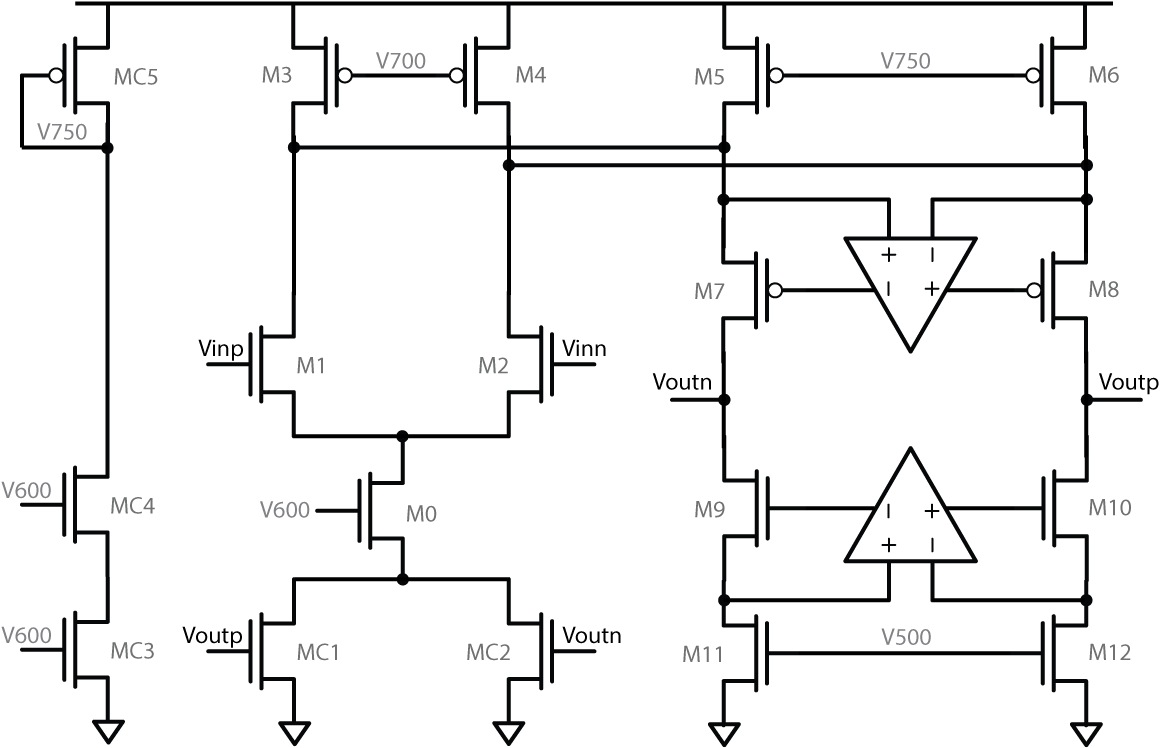
\includegraphics[width=\linewidth]{illus/main_ota}
\caption{Gain-boosted folded cascode OTA with CMFB}
\label{fig:main-ota}
\end{figure}

\begin{center}
\begin{tabular}{|c|c|c|c|c|c|c|} 
\hline
Device & W ($\mu$) & L (n) & V* & $I_D$(m) & $g_m$(m) & $f_T$(G) \\
\hline
\multicolumn{7}{|c|}{Differential pair} \\
\hline
M0 &	 42.1 & 90 & 0.22 & 3.63 & 33 & 94.7 \\
\hline
M1/2 &  15.9 & 60 & 0.20 & 1.81 & 18.4 & 224 \\
\hline
M3/4 & 154.8 & 100 & 0.19 & 1.81 & 19 & 13.4 \\
\hline
\multicolumn{7}{|c|}{Output branch} \\
\hline
M5/6 & 172.98 & 80 & 0.15 & 1.8 & 23.5 & 20.2 \\
\hline
M7/8 & 79.38 & 100 & 0.25 & 1.77 & 14.3 & 18.3 \\
\hline
M9/10 & 71.35 & 300 & 0.19 & 1.77 & 18.8 & 97.2 \\
\hline
M11/12 & 88.56 & 200 & 0.15 & 1.45 & 23.3 & 17.2 \\ %Pm77
\hline
\multicolumn{7}{|c|}{CMFB} \\
\hline
MC1/2 & 15.13 & 60 & 0.7 & 1.81 & 5.1 & 57.3 \\
\hline
MC3 & 12.61 & 60 & 0.6 & 1.52 & 5.1 & 68.7 \\
\hline
MC4 & 14.5 & 90 & 0.22 & 1.52 & 13.7 & 112 \\
\hline
MC5 & 195.3 & 140 & 0.14 & 1.52 & 21.4 & 5.02 \\
\hline
\end{tabular}
\end{center}


\begin{figure}[h]
\centering
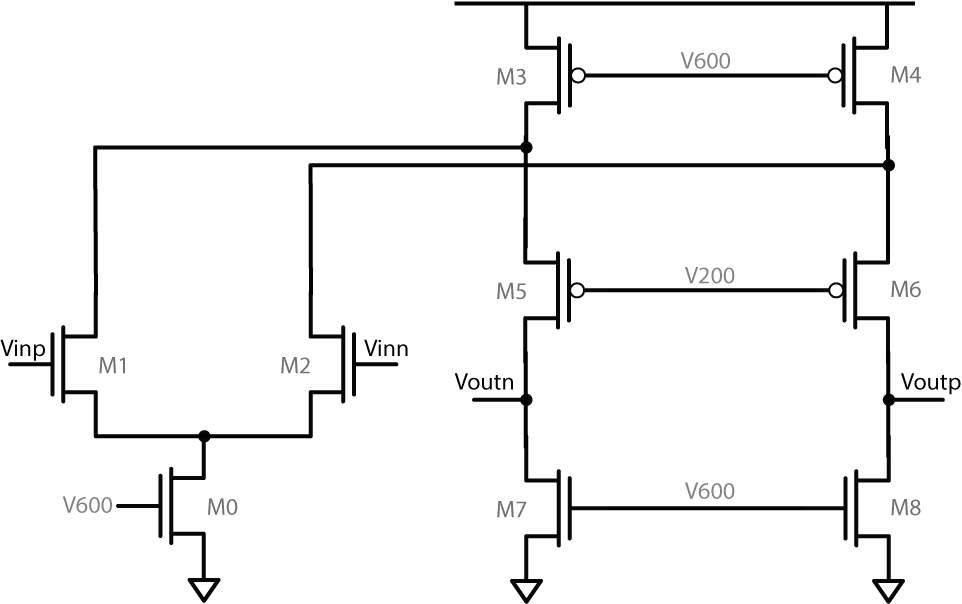
\includegraphics[width=0.75\linewidth]{illus/pmos_boost}
\caption{PMOS Gain Booster}
\label{fig:pmos_boost}
\end{figure}

\begin{center}
\begin{tabular}{|c|c|c|c|c|c|c|} 
\hline
Device & W ($\mu$) & L (n) & V* & $I_D$(m) & $g_m$(m) & $f_T$(G) \\
\hline
\multicolumn{7}{|c|}{Differential pair} \\
\hline
M0 &	 16.4 & 90 & 0.29 & 2 & 13.9 & 122.7 \\
\hline
M1/2 &  14 & 90 & 0.14 & 1 & 14.2 & 78 \\
\hline
\multicolumn{7}{|c|}{Output branch} \\
\hline
M3/4 & 11.6 & 90 & 0.3 & 1.5 & 10.1 & 26.4 \\
\hline
M5/6 & 2.6 & 90 & 0.4 & 0.5 & 2.53 & 108 \\
\hline
M7/8 & 4 & 100 & 0.28 & 0.5 & 3.5 & 89 \\
\hline
\end{tabular}
\end{center}


\begin{figure}[h]
\centering
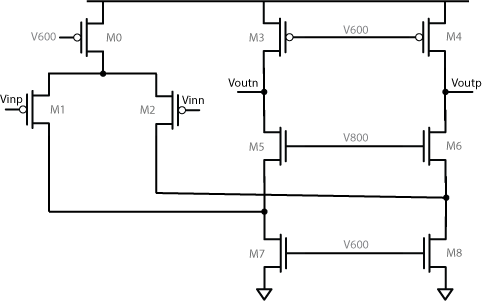
\includegraphics[width=0.75\linewidth]{illus/nmos_boost}
\caption{NMOS Gain Booster}
\label{fig:nmos_boost}
\end{figure}

\begin{center}
\begin{tabular}{|c|c|c|c|c|c|c|} 
\hline
Device & W ($\mu$) & L (n) & V* & $I_D$(m) & $g_m$(m) & $f_T$(G) \\
\hline
\multicolumn{7}{|c|}{Differential pair} \\
\hline
M0 &	 198.4 & 200 & 0.27 & 2.2 & 16 & 3.98 \\
\hline
M1/2 &  77.5 & 60 & 0.13 & 1.1 & 16.3 & 43 \\
\hline
\multicolumn{7}{|c|}{Output branch} \\
\hline
M3/4 & 68.5 & 150 & 0.28 & 1.1 & 7.95 & 7.6 \\
\hline
M5/6 & 49.7 & 100 & 0.13 & 1.1 & 17.3 & 58 \\
\hline
M7/8 & 7.13 & 60 & 0.44 & 2.2 & 10.1 & 237 \\
\hline
\end{tabular}
\end{center}


\begin{figure}[h]
\centering
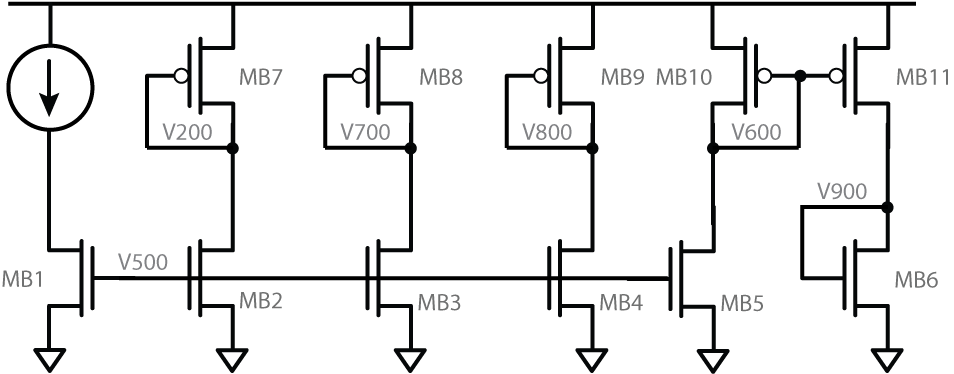
\includegraphics[width=0.75\linewidth]{illus/bias}
\caption{Biasing Network}
\label{fig:bias}
\end{figure}

\begin{center}
\begin{tabular}{|c|c|c|c|c|c|c|} 
\hline
Device & W ($\mu$) & L (n) & V* & $I_D$(m) & $g_m$(m) & $f_T$(G) \\
\hline
MB1 & 5.89 & 80 & 0.19 & 0.5 & 5.27 & 128 \\
\hline
MB2 & 7.18 & 80 & 0.18 & 0.5 & 5.6 & 115 \\
\hline
MB3 & 5.27 & 80 & 0.18 & 0.5 & 5.6 & 115\\
\hline
MB4 & 4.99 & 80 & 0.18 & 0.5 & 5.6 & 115\\
\hline
MB5 & 5.56 & 80 & 0.18 & 0.5 & 5.6 & 115\\
\hline
MB6 & 2.69 & 300 & 0.65 & 0.5 & 1.54 & 17.5 \\
\hline
MB7 & 2.6 & 140 & 0.83 & 0.5 & 1.2 & 88.9 \\
\hline
MB8 & 34 & 140 & 0.18 & 0.5 & 5.6 & 6.5 \\
\hline
MB9 & 142.59 & 140 & 0.12 & 0.5 & 8.6 & 3.82 \\
\hline
MB10 & 13.7 & 140 & 0.28 & 0.5 & 3.57 & 9.17 \\
\hline
MB11 & 14.5 & 140 & 0.28 & 0.5 & 3.57 & 9.17 \\
\hline
\end{tabular}
\end{center}


\section{Design Verification}

The spec specified that the OTA would be used in a delta-sigma ADC with a +/-1V differential square wave from the D/A. Therefore, we assumed that the settling time needed to be met, at worst, for a 1V differential input signal. So with a gain of .5, the output needed to settle to .5V differential in 1.8ns. This is how we determined that our settling and dynamic error met spec in fig. \ref{fig:st1_error}.

Running transient on a 1V step after enough time for the common mode feedback was the ultimate verification of our design, but stability analysis was the first check of our design to make sure that the transient would be stable and the settling time would meet. Stability sims were run on the gain boosters, the common mode feedback loop, and the OTA constant time integrator loop of both stages.

Stability analysis in figs. \ref{fig:st1_diff_ac}, \ref{fig:st1_cm_ac}, \ref{fig:st2_diff_ac} and \ref{fig:st2_cm_ac} shows that indeed, the unity gain bandwidth and phase margin requirements are met and surpassed for both the first and second stages. We originally had some trouble with stability from the gain boosters, and the Phase Margin report from the stability analysis was very necessary to verify before using the gain boosters in the larger circuit. The common mode feedback loop is included as well because the integrator is unstable for phase margin of less than 45 degrees, which is not reflected in the differential loop analysis.



The transient simulation was used to verify that the output settled to within 0.1 percent at 1.8ns. We plotted both the differential output and separate outputs. Settling is easily verified from the differential output in figs. \ref{fig:st1_error} and \ref{fig:st2_error}, and common mode output is seen in figs. \ref{fig:st1_trans} and \ref{fig:st2_trans}. This figure shows that there is some common mode settling that occurs immediately after switching, which is not reflected in the differential. Both stages are verified in this manner, and meet spec.

In addition, transient was used to examine the effect of slewing on the 1V step settling. As you can see in the final transient simulation in fig. \ref{fig:st1_slew}, the highlighted line is the output current which is constant as the circuit supplies the entire 1.6mA that is can before it is no longer biased properly. The slewing occurs for the .5ns that is was allotted for settling.

Finally, to determine that the noise spec was met, we ran noise sims over 1600 sidebands and 400 harmonics. We used ideal switches instead of transistors, but used series resistors to simulate noise from switch resistance. We input referred the noise to obtain the values seen in the results.\\

\section{Final Specification}

\begin{center}
\begin{tabular}{|c|c|} 
\hline
Gain & 0.5 \\
\hline
Input Referred Noise & 9.18 $\mu$ $V_{RMS}$ \\
\hline
Settling & 0.1\% in 1.27 ns \\
\hline
Sampling Freq & 250MHz \\
\hline
Total Power & 43.056 mW \\
\hline
\end{tabular}
\end{center}

1st stage noise 8.86uV
2nd stage noise 0.31950uV
19.09 mA 1st stage
13.79 mA 2nd stage
3mA biasing
35.88 mA totall

\section{Design Critique}

Our integrator circuit is over designed. We settle faster than the required spec and have lower noise than required. The circuit has a large footprint and burns more power than necessary to do this. We could have traded some power to more closely meet specs, especially in the second stage, where we had to add a load cap in order to get the necessary phase margin. If power was a tight spec, then we would have done this, but considering variation across the die and across chips, we decided that it was better to overshoot and make a circuit that is more easily built and with a better yield. This is especially important for our circuit because we chose very particular widths and lengths for our mosfets, which makes the circuit harder to actualize in silicon. Variation would have a large effect, so a little over-design is not a huge problem if the power budget can afford it. If we had more time we would have continued to tweak values and biases to see if we could obtain the same performance for lower power.

Second, our design did not take flicker noise into account. If we had, then our larger width and higher power would have been an advantage, but we assumed that since this was for an ADC application it was typical to add a chopper and then flicker would not be a concern.

Our design did not do anything to correct for offset, which might be a concern because our input devices are a bit small and thus variation would have a significant effect. However, considering that the application is an ADC this is not too concerning because the effect of OTA offset from fabrication mismatch is negligible because Delta-Sigma modulators are relatively insensitive to offset [1].





\begin{figure*}[H]
\centering
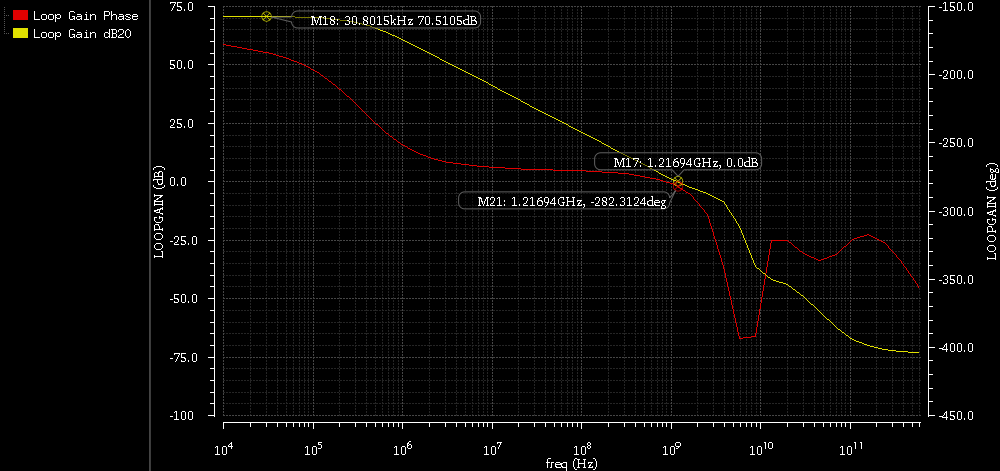
\includegraphics[height=250px]{piktures/st1_diff_ac}
\caption{Stability Analysis simulation of the differential loop for the first stage}
\label{fig:st1_diff_ac}
\end{figure*}

\begin{figure*}[H]
\centering
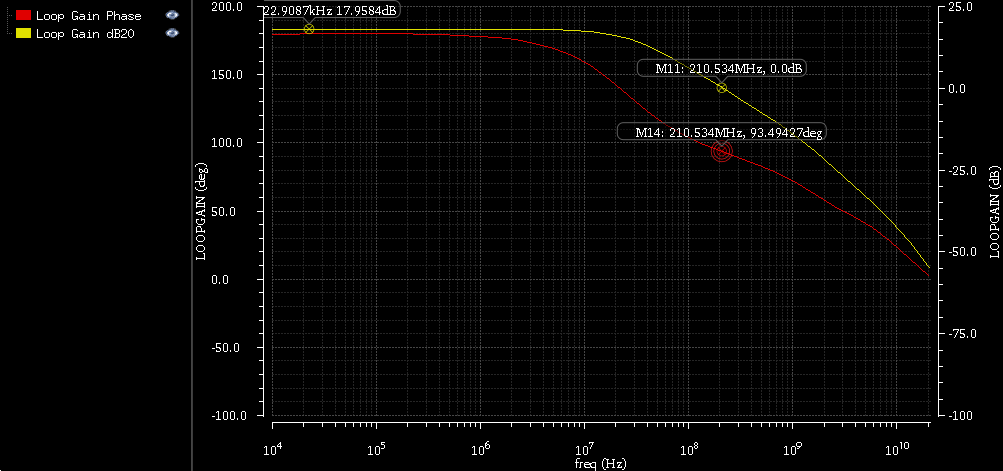
\includegraphics[height=250px]{piktures/st1_cm_ac}
\caption{Stability Analysis simulation of the common mode loop for the first stage}
\label{fig:st1_cm_ac}
\end{figure*}

\begin{figure*}[H]
\centering
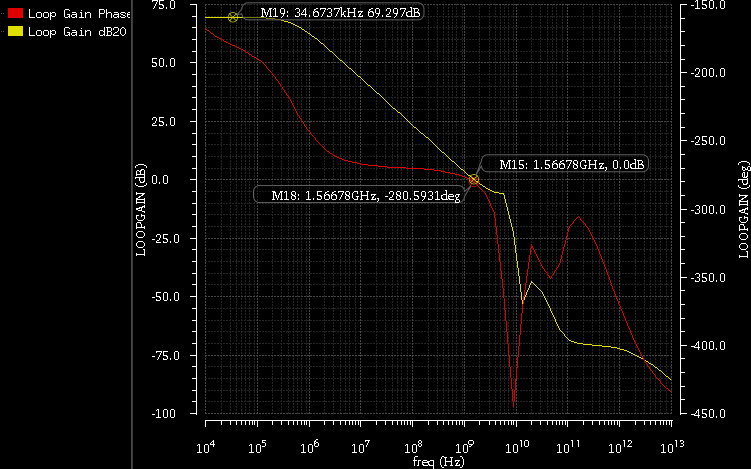
\includegraphics[height=250px]{piktures/st2_diff_ac}
\caption{Stability Analysis simulation of the differential loop for the first stage}
\label{fig:st2_diff_ac}
\end{figure*}

\begin{figure*}[H]
\centering
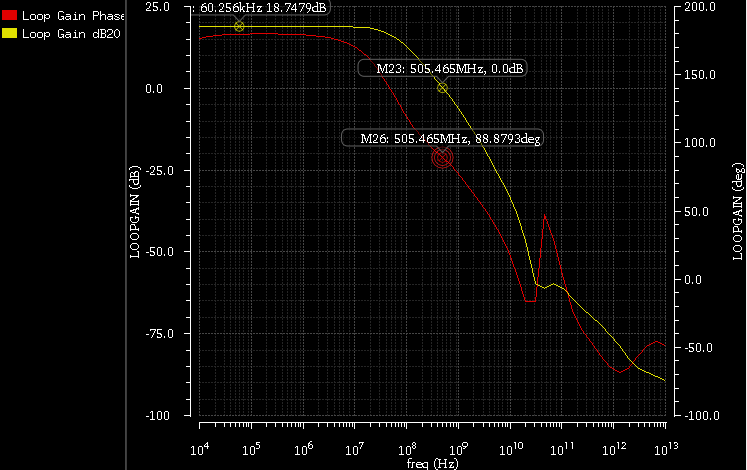
\includegraphics[height=250px]{piktures/st2_cm_ac}
\caption{Stability Analysis simulation of the common mode loop for the first stage}
\label{fig:st2_cm_ac}
\end{figure*}




\begin{figure*}[H]
\centering
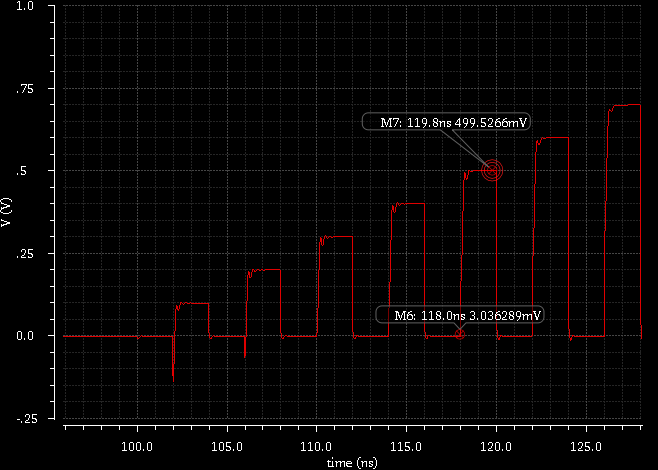
\includegraphics[height=250px]{piktures/st1_error}
\caption{Transient settling error of first integrator for a 100mV input}
\label{fig:st1_error}
\end{figure*}

\begin{figure*}[H]
\centering
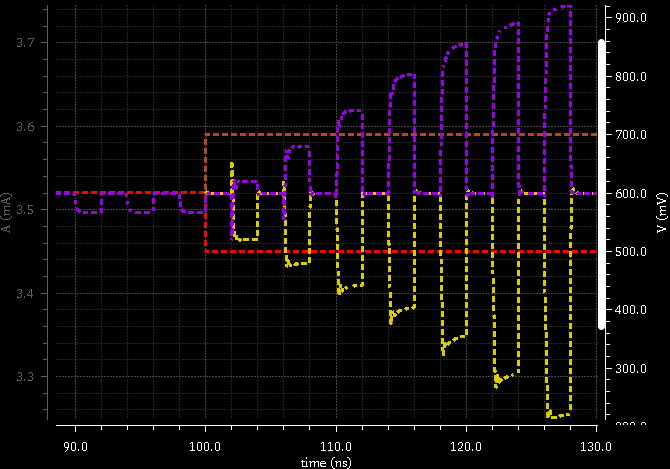
\includegraphics[height=250px]{piktures/st1_trans}
\caption{Transient response of first integrator for a 100mV input}
\label{fig:st1_trans}
\end{figure*}

\begin{figure*}[H]
\centering
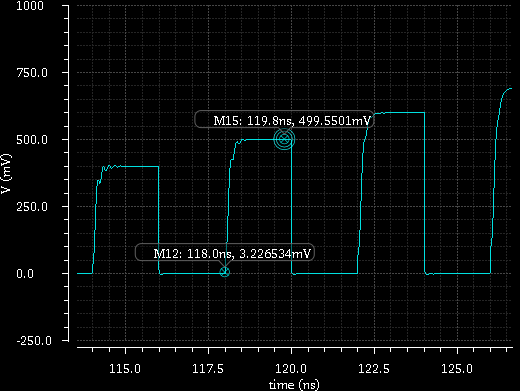
\includegraphics[height=250px]{piktures/st2_error}
\caption{Transient settling error of first integrator for a 100mV input}
\label{fig:st2_error}
\end{figure*}

\begin{figure*}[H]
\centering
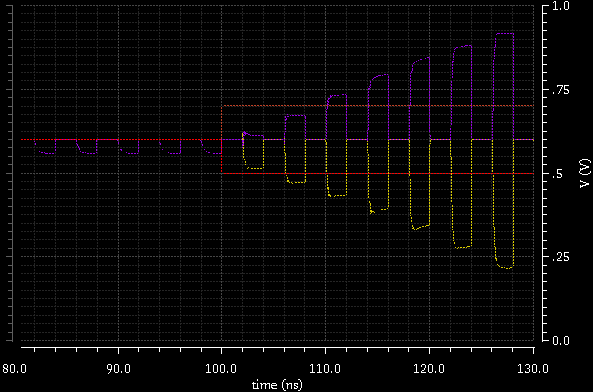
\includegraphics[height=250px]{piktures/st2_trans}
\caption{Transient response of first integrator for a 100mV input}
\label{fig:st2_trans}
\end{figure*}

\begin{figure*}[H]
\centering
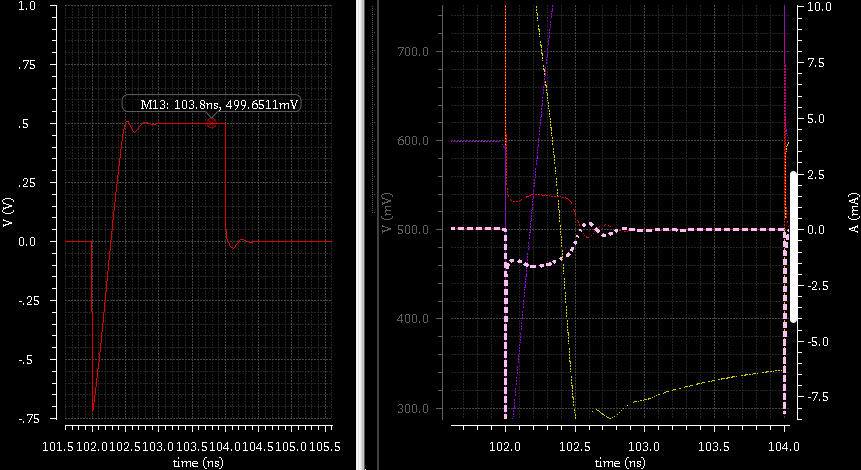
\includegraphics[height=250px]{piktures/st1_slew}
\caption{Transient response of first integrator for a 1V input showing slewing}
\label{fig:st1_slew}
\end{figure*}















\begin{comment}


\section{Design}
For this project the important specifications are:

\begin{center}
\begin{tabular}{|c|c|} 
\hline
Gain (Stage 1) & 0.5 \\
\hline
Input Referred Noise & $10\mu$ $V_{RMS}$ \\
\hline
Settling & 0.1\% in 1.8ns \\
\hline
Sampling Freq & 250M Hz \\
\hline
\end{tabular}
\end{center}

We divided the settling error requirement evenly between static and dynamic error, so $\epsilon_d = 0.05\%$. Furthermore, we decided to budget noise based on the noise factor calculations from the previous section. We see that the noise $\phi_1$ is the most important contribution to the noise. $\phi_2$ will be divided by a factor of 1000, therefore budget nearly all of the noise requirements for noise from $N_{11}$. The spec is for differential noise, so calculating single ended, we need to hit $5\mu$ $V_{RMS}$. We divide that further up, so that there is $3\mu$ $V_{RMS}$ for one input of the first integrator, and $1\mu$ $V_{RMS}$ for one input of the second stage and output of the second stage, taking advantage of the fact that the second integrator can be designed with much looser noise requirements.

From these specifications, we see that the small noise and rapid settling time will require careful design to meet both simultaneously. We began by considering a basic switched capacitor integrator in fig. \ref{int1} to get an idea of the what values were needed to meet $3\mu$ $V_{RMS}$ per input. We can use a design process similar to that of a sample and hold circuit, with only minor differences due to different switches.

\begin{figure}[h]
\centering
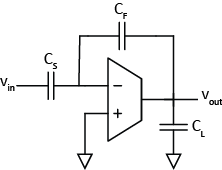
\includegraphics[width=0.4\linewidth]{illustrator/integrator1}
\caption{Basic switched capacitor gain stage}
\label{int1}
\end{figure}

The necessary equations are below. \newline
Gain:
$$\frac{V_{out}}{V_{in}}=\frac{C_S}{C_F}$$
Settling Time:
$$t_s = -\tau ln \left(\epsilon_d \left(1-\beta \frac{C_F}{C_F-C_L}\right)\right)$$
Noise:
$$N_{\phi 1} = \frac{kT}{C_S + C_L}$$
$$N_{\phi 2} = \frac{\alpha}{\beta}\frac{kT}{C_{L,tot}}$$
Where in these equations $\alpha$ is the noise factor of the OTA - we used $\alpha = 2$ for the design - and $\beta$ is the feedback factor. $$\beta = \frac{C_F}{C_S + C_F + C_L}$$ 
In addition, $C_{L,tot}$ is the effective capacitive load.$$C_{L,tot}=C_L+(1-\beta)C_F$$
And $\tau$ is the time constant of the system. $$\tau = \frac{C_{L,tot}}{\beta G_m}$$

\subsection{First Integrator Stage}

We begin by choosing $C_S$ from the noise spec and the equation for $\phi_1$. Then $C_F$ is easily obtained from the required gain. We want to meet $3\mu$ $V_{RMS}$ per input, but the BW that we care about noise is only 100-500kHz and our equation for $N_{\phi 1}$ is over the entire spectrum [1]. Therefore, we need to multiply the noise spec by the Oversampling Ratio, which is $\frac{f_S}{2BW}$. The noise that we want at the input therefore is $N_{11}=250 \cdot 9\cdot 10^{-12} V/\sqrt{Hz}$.
%IMPT VALS
$$C_S = 2pF$$ 
$$C_F = 4pF$$
These are somewhat large capacitor values to drive. We next calculate the $G_m$ of the OTA necessary to meet the settling time with those capacitors from $\tau$. We get $G_m = 9mS$, which is a little large, but should be doable with large width MOSFETs.
We began adding parasitics to the transconductor. Parasitic capacitors are from $C_{GS}=\frac{g_m}{\omega_T}$ and we made a first optimistic guess at a conservative $r_o=10k$ and found that in simulation we needed significantly larger $G_m$. A small $G_m$ would result in a small loop gain due to the non-infinite $r_o$, which creates a significant static settling error.
We decided that $G_m$ was getting a little large and decided to check a cascaded setup shown in fig. \ref{int2}. 

\begin{figure}[h]
\centering
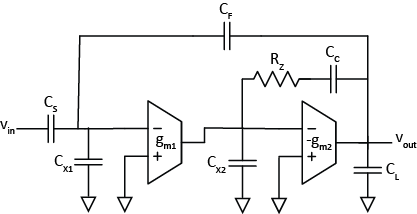
\includegraphics[width=0.7\linewidth]{illustrator/integrator2}
\caption{Cascaded amplifiers with Miller compensation}
\label{int2}
\end{figure}
 
The relevant equations for this part change only a little:
$$\tau = \frac{C_C}{\beta g_{m1}}$$
$$N_{\Phi 2} = \frac{\alpha_1}{\beta} \frac{kT}{C_C} \left( 1+\beta \frac{\alpha_2}{\alpha_1} \frac{C_C}{C_{Ltot}} \right)$$

However, most of the equations for poles and zeros are very approximated, and they do not take into account that the cascaded amplifiers are more stable when $g_{m1}$ is larger than $g_{m2}$. We also had to use a Miller capacitance for pole splitting.

We had to iteratively find a stable value of $g_m$s that met timing, and eventually settled on $g_{m1}=20mS$, $g_{m2}=4mS$.

\begin{figure}[h]
\centering
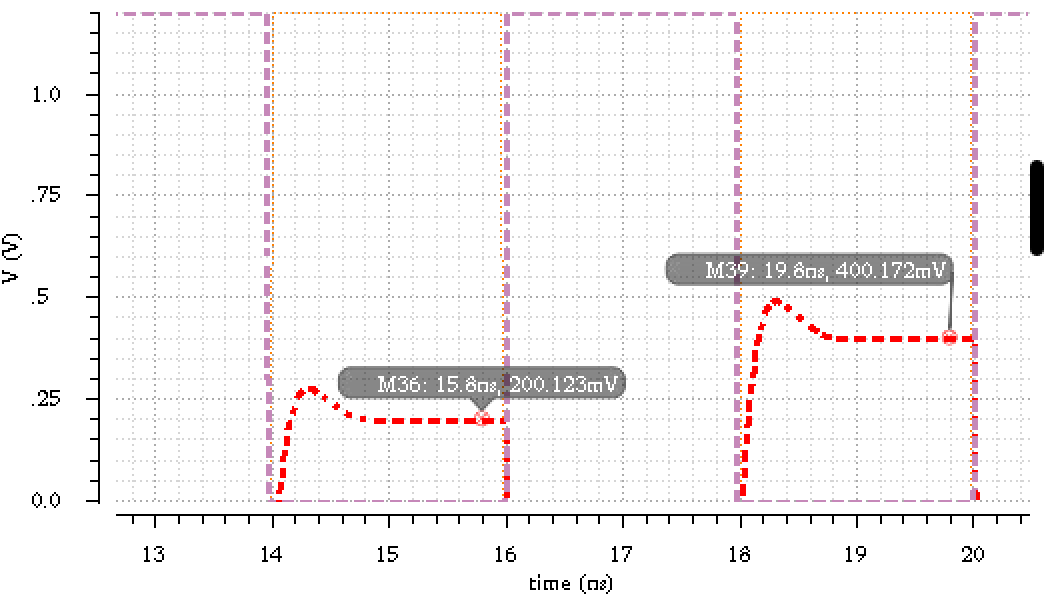
\includegraphics[width=\linewidth]{img/cascaded-tran}
\caption{Transient response of 2-stage amplifier with Miller compensation}
\label{cascaded-tran}
\end{figure}

These value of $g_m$ are not significantly better than the single stage transconductor and the noise of a single stage is better, so we decided that a very large diff pair would be better than cascading.

We re-examined the parasitic resistance and decided that increasing the $r_o$ was the next best option, so that we needed the first stage OTA to be a single stage diff pair with cascoding, and approximated the new $r_o$ as a conservative $100k\Omega$.

We ran a final transient sim to make sure that the settling time of the output of the first stage was 1.8ns to 0.1\%. 

\begin{figure}[h]
\centering
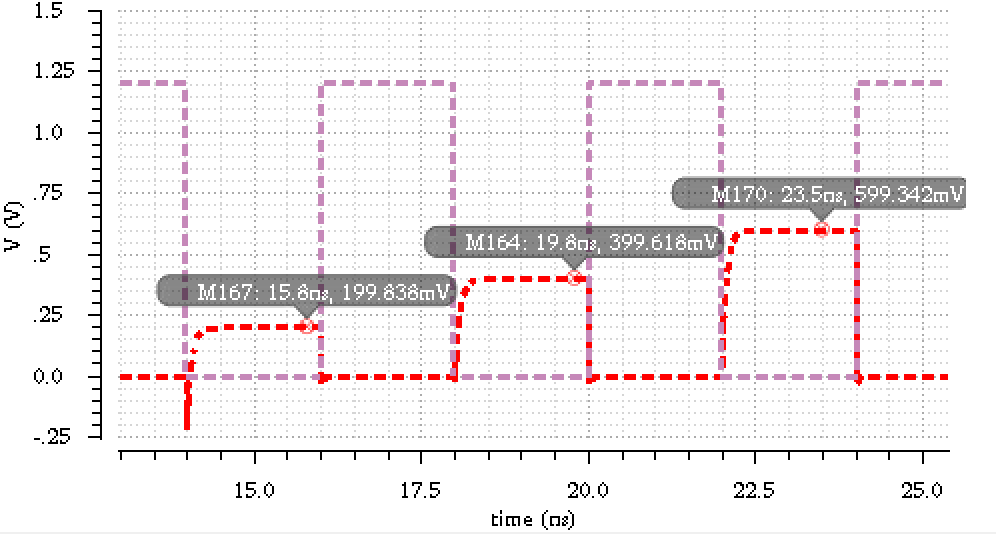
\includegraphics[width=\linewidth]{img/stage1-tran}
\caption{Transient response of first integrator with single-stage amplifier}
\label{stage1-tran}
\end{figure}

The noise simulation was a performed with a noise current source from a resistor of value $\frac{\alpha}{G_m}$ inside of the OTA and $10\Omega$ ON resistances in series with all of the switches. However, PSS and PNOISE are not really meant for integrators so we exported the noise density at the output of the integrator to Matlab, then multiplied by the transfer function from the noise source $N_{12}$ to the input and then integrated over the BW.

\begin{figure}[h]
\centering
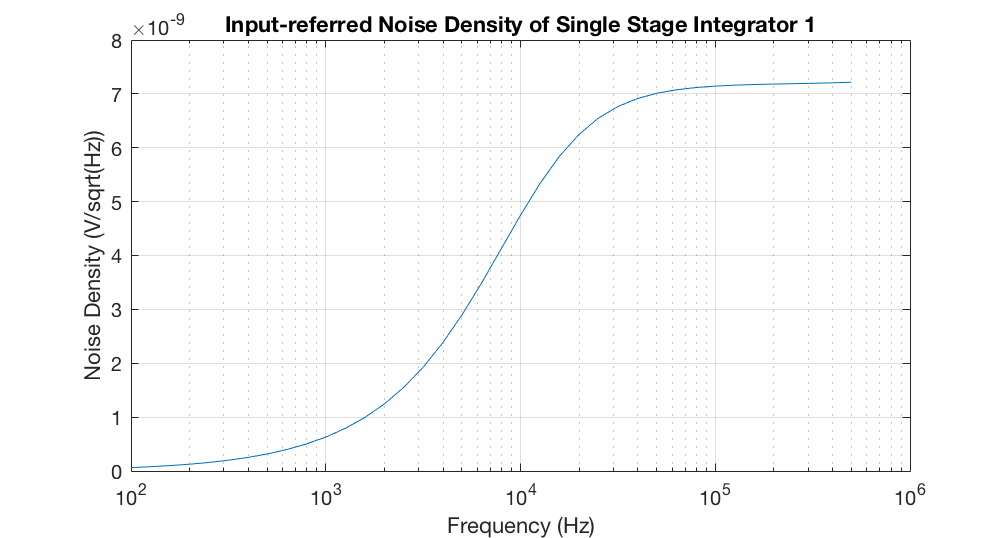
\includegraphics[width=\linewidth]{img/noise-stage1}
\caption{Input-referred noise density from the first integrator stage}
\label{noise-stage1}
\end{figure}

The integrated noise is $2.245\mu V_{RMS}$ which gives us a lot of room to change $C_s$ if we need it.

\begin{center}
\begin{tabular}{|c|c|} 
\hline
$C_S$ & 2pF \\
\hline
$C_F$ & 4pF \\
\hline
$G_M$ & 19mS \\
\hline
$R_{o,min}$ & 100k$\Omega$ \\
\hline
\end{tabular}
\end{center}

In this stage, the most important design factor is meeting the noise requirement. This means that if noise is a problem later in the problem we can increase $C_S$. However, since we are very cleanly meeting the noise spec, we can trade some of it for lower $G_m$ in the gain stage. The large capacitors in the feedback loop relative to the load capacitance of the next stage mean we don't need quite as good of output resistance to keep static error within spec.

\subsection{Second Integrator Stage}

For second stage, we are meeting a noise spec which is 1000 times more lenient. Thus, we can choose much smaller feedback capacitance and $G_m$ of the OTA can be much more lenient. Using the same design procedure as before we obtain the values for the second integrator, also with a gain of 0.5. A larger gain would marginally help with the noise requirements, but a smaller gain would result in a higher $\beta$, hence higher loop gain. This is required once we have some load resistance at the output to meet the static settling error with a reasonable $G_m$.

\begin{center}
\begin{tabular}{|c|c|} 
\hline
$C_S$ & 30fF \\
\hline
$C_F$ & 15fF \\
\hline
$G_M$ & 5mS \\
\hline
$R_{o,min}$ & 1M$\Omega$ \\
\hline
\end{tabular}
\end{center}


We did find, that because the feedback capacitors are not on the same order as the load cap, the static error is a much bigger concern, so we need to meet a larger output resistance of the OTA in order to keep the $g_m$ build-able with one stage.

\begin{figure}[h]
\centering
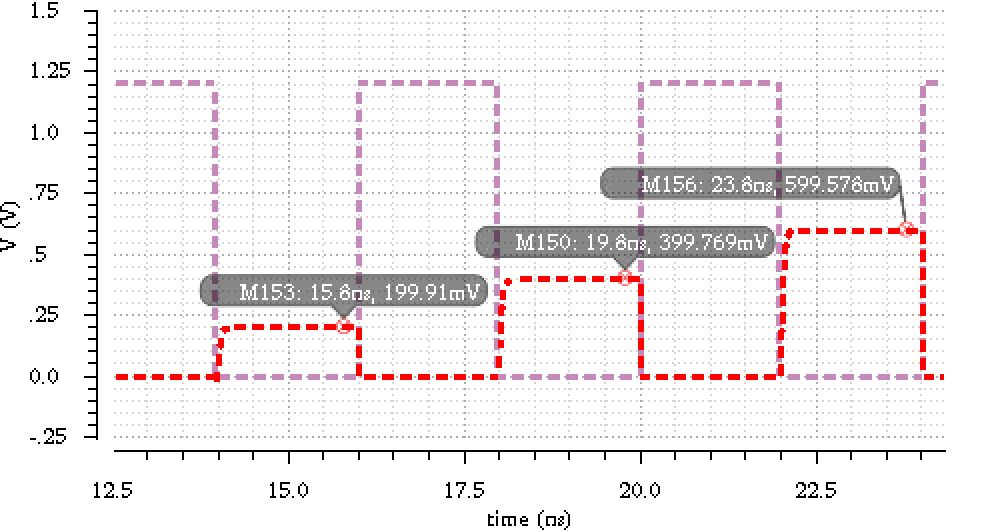
\includegraphics[width=\linewidth]{img/stage2-tran}
\caption{Transient response of second integrator with single-stage amplifier}
\label{stage2-tran}
\end{figure}

\begin{figure}[h]
\centering
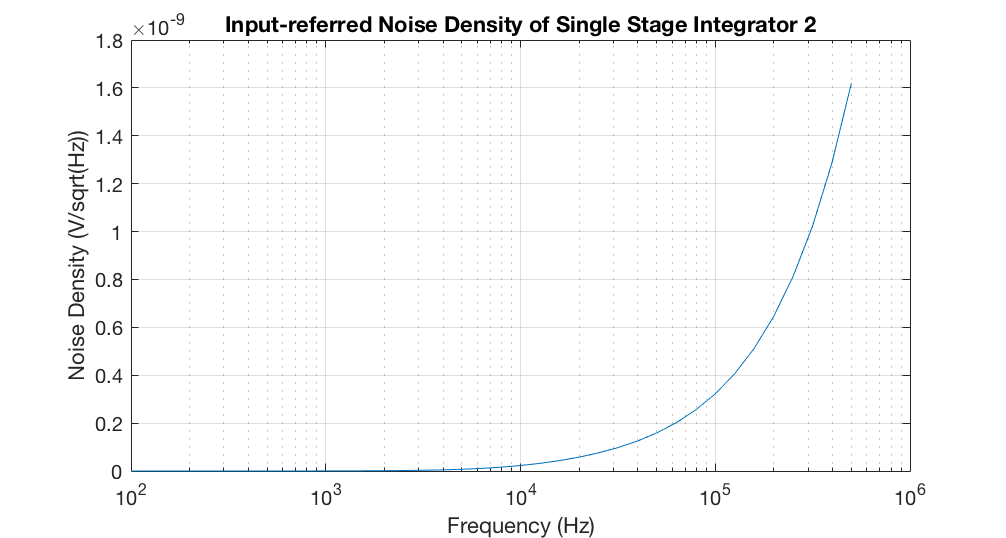
\includegraphics[width=\linewidth]{img/noise-stage2}
\caption{Input-referred noise density from the second integrator stage}
\label{noise-stage2}
\end{figure}


\section{Implementation}

\subsection{OTAs}
The above simulations confirmed that we needed reasonably large $G_m$ OTAs, and that output resistance is more important for the second stage than the first stage.

\begin{figure}[h]
\centering
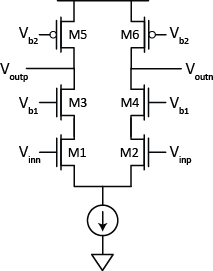
\includegraphics[width=0.4\linewidth]{illustrator/cascoded-diffpair}
\caption{Cascoded fully-differential pair}
\label{cascoded-diffpair}
\end{figure}

For the first stage we want a differential pair with reasonably large output resistance. We propose the cascoded fully-differential pair in fig. \ref{cascoded-diffpair}.
$M_1$ and $M_2$ completely determine the $G_m$ of the OTA and will need to be sized accordingly. The large width of $M_1$ and $M_2$ necessitates using cascoding at least on the input caps, but careful sizing of $M_5$ and $M_6$ should meet the required output resistance of the first stage without having to use a full telescopic design which will limit the output swing a lot.

For the second stage, however, we need better output resistance, in which case we need a telescopic differential pair, but we should not need gain boosting. The output voltage swing is not defined in the spec, so cascoded devices is feasible.

\subsection{Switches}
The resistance of the switches is somewhat of a concern, especially for the sampling switch. The time constant of this switch with $C_S$ needs to be substantially low such that the sampling capacitor has time to charge sufficiently, and that the switch can drive over the large input range. Therefore, the first switch, at least, needs to be a reasonably wide transmission gate.

The problem with large switches is that they have a lot of charge injection. To avoid that, we are making sure that we use early switches to disconnect the sampling cap and to implement bottom plate sampling.

\begin{figure}[h]
\centering
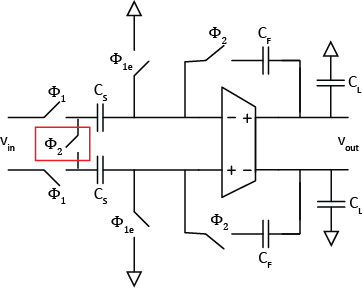
\includegraphics[width=0.8\linewidth]{illustrator/integrator3}
\caption{Integrator stage with added features}
\label{integrator3}
\end{figure}


\subsection{Integrators}
At the integrator level, we have been dealing only with the specs for this project. The project does not specify a CMRR or amount of variation that we have to be able to deal with in fabrication. However, these are things that have to be dealt with.

We propose the integrator implementation in fig.\ref{integrator3} to deal with problems outside of simulation.

The switch between the inputs to the OTA marked with the red box is to improve the CMRR by canceling the common mode offset [2]. The effect of OTA offset from fabrication mismatch is negligible because Delta-Sigma modulators are relatively insensitive to offset [3].


\end{comment}


%\subsection{Subsection Heading Here}
%Subsection text here.


%\subsubsection{Subsubsection Heading Here}
%Subsubsection text here.


% An example of a floating figure using the graphicx package.
% Note that \label must occur AFTER (or within) \caption.
% For figures, \caption should occur after the \includegraphics.
% Note that IEEEtran v1.7 and later has special internal code that
% is designed to preserve the operation of \label within \caption
% even when the captionsoff option is in effect. However, because
% of issues like this, it may be the safest practice to put all your
% \label just after \caption rather than within \caption{}.
%
% Reminder: the "draftcls" or "draftclsnofoot", not "draft", class
% option should be used if it is desired that the figures are to be
% displayed while in draft mode.
%
%\begin{figure}[!t]
%\centering
%\includegraphics[width=2.5in]{myfigure}
% where an .eps filename suffix will be assumed under latex, 
% and a .pdf suffix will be assumed for pdflatex; or what has been declared
% via \DeclareGraphicsExtensions.
%\caption{Simulation results for the network.}
%\label{fig_sim}
%\end{figure}

% Note that the IEEE typically puts floats only at the top, even when this
% results in a large percentage of a column being occupied by floats.


% An example of a double column floating figure using two subfigures.
% (The subfig.sty package must be loaded for this to work.)
% The subfigure \label commands are set within each subfloat command,
% and the \label for the overall figure must come after \caption.
% \hfil is used as a separator to get equal spacing.
% Watch out that the combined width of all the subfigures on a 
% line do not exceed the text width or a line break will occur.
%
%\begin{figure*}[!t]
%\centering
%\subfloat[Case I]{\includegraphics[width=2.5in]{box}%
%\label{fig_first_case}}
%\hfil
%\subfloat[Case II]{\includegraphics[width=2.5in]{box}%
%\label{fig_second_case}}
%\caption{Simulation results for the network.}
%\label{fig_sim}
%\end{figure*}
%
% Note that often IEEE papers with subfigures do not employ subfigure
% captions (using the optional argument to \subfloat[]), but instead will
% reference/describe all of them (a), (b), etc., within the main caption.
% Be aware that for subfig.sty to generate the (a), (b), etc., subfigure
% labels, the optional argument to \subfloat must be present. If a
% subcaption is not desired, just leave its contents blank,
% e.g., \subfloat[].


% An example of a floating table. Note that, for IEEE style tables, the
% \caption command should come BEFORE the table and, given that table
% captions serve much like titles, are usually capitalized except for words
% such as a, an, and, as, at, but, by, for, in, nor, of, on, or, the, to
% and up, which are usually not capitalized unless they are the first or
% last word of the caption. Table text will default to \footnotesize as
% the IEEE normally uses this smaller font for tables.
% The \label must come after \caption as always.
%
%\begin{table}[!t]
%% increase table row spacing, adjust to taste
%\renewcommand{\arraystretch}{1.3}
% if using array.sty, it might be a good idea to tweak the value of
% \extrarowheight as needed to properly center the text within the cells
%\caption{An Example of a Table}
%\label{table_example}
%\centering
%% Some packages, such as MDW tools, offer better commands for making tables
%% than the plain LaTeX2e tabular which is used here.
%\begin{tabular}{|c||c|}
%\hline
%One & Two\\
%\hline
%Three & Four\\
%\hline
%\end{tabular}
%\end{table}


% Note that the IEEE does not put floats in the very first column
% - or typically anywhere on the first page for that matter. Also,
% in-text middle ("here") positioning is typically not used, but it
% is allowed and encouraged for Computer Society conferences (but
% not Computer Society journals). Most IEEE journals/conferences use
% top floats exclusively. 
% Note that, LaTeX2e, unlike IEEE journals/conferences, places
% footnotes above bottom floats. This can be corrected via the
% \fnbelowfloat command of the stfloats package.




% conference papers do not normally have an appendix


% use section* for acknowledgment
%\section*{Acknowledgment}


%The authors would like to thank...





% trigger a \newpage just before the given reference
% number - used to balance the columns on the last page
% adjust value as needed - may need to be readjusted if
% the document is modified later
%\IEEEtriggeratref{8}
% The "triggered" command can be changed if desired:
%\IEEEtriggercmd{\enlargethispage{-5in}}

% references section

% can use a bibliography generated by BibTeX as a .bbl file
% BibTeX documentation can be easily obtained at:
% http://mirror.ctan.org/biblio/bibtex/contrib/doc/
% The IEEEtran BibTeX style support page is at:
% http://www.michaelshell.org/tex/ieeetran/bibtex/
%\bibliographystyle{IEEEtran}
% argument is your BibTeX string definitions and bibliography database(s)
%\bibliography{IEEEabrv,../bib/paper}
%
% <OR> manually copy in the resultant .bbl file
% set second argument of \begin to the number of references
% (used to reserve space for the reference number labels box)


\begin{thebibliography}{1}

\begin{comment}

\bibitem{}
R. Schreier, \emph{Design-Oriented Estimation of Thermal Noise in Switched-Capacitor Circuits},  IEEE Transactions on Circuits and Systems—I: Regular Papers, vol.52, no.11, 2005.

\bibitem{}
S. Lewis, P. Gray. \emph{A Pipelined 5-Msample/s 9-bit Analog-to-Digital Converter}, IEEE Journal of Solid-State Circuits, vol.sc-22 ,no.6, 1987.

\end{comment}

\bibitem{}
B. Bernhard, \emph{The Design of Sigma-Delta Modulation Analog-to-Digita1 Converters}, IEEE Journal of Solid-State Circuits, vol.23 ,no.6, 1988.

\end{thebibliography}

% that's all folks
\end{document}
